\documentclass{scrbook}

%!TEX root = thesis.tex

% Set german to default language and load english as well
\usepackage[english,ngerman]{babel}

% Set UTF8 as input encoding
\usepackage[utf8]{inputenc}

% Set T1 as font encoding
\usepackage[T1]{fontenc}
% Load a slightly more modern font
\usepackage{lmodern}
% Use the symbol collection textcomp, which is needed by listings.
\usepackage{textcomp}
% Load a better font for monospace.
\usepackage{courier}

% Set some options regarding the document layout. See KOMA guide
\KOMAoptions{%
  paper=a4,
  fontsize=12pt,
  parskip=half,
  headings=normal,
  BCOR=1cm,
  headsepline,
  DIV=12}

% do not align bottom of pages
\raggedbottom

% set style of captions
\setcapindent{0pt} % do not indent second line of captions
\setkomafont{caption}{\small}
\setkomafont{captionlabel}{\bfseries}
\setcapwidth[c]{0.9\textwidth}

% set the style of the bibliography
\bibliographystyle{alphadin}

% load extended tabulars used in the list of abbreviation
\usepackage{tabularx}

% load the color package and enable colored tables
\usepackage[table]{xcolor}

% define new environment for zebra tables
\newcommand{\mainrowcolors}{\rowcolors{1}{maincolor!25}{maincolor!5}}
\newenvironment{zebratabular}{\mainrowcolors\begin{tabular}}{\end{tabular}}
\newcommand{\setrownumber}[1]{\global\rownum#1\relax}
\newcommand{\headerrow}{\rowcolor{maincolor!50}\setrownumber1}

% add main color to section headers
\addtokomafont{chapter}{\color{maincolor}}
\addtokomafont{section}{\color{maincolor}}
\addtokomafont{subsection}{\color{maincolor}}
\addtokomafont{subsubsection}{\color{maincolor}}
\addtokomafont{paragraph}{\color{maincolor}}

% do not print numbers next to each formula
\usepackage{mathtools}
\mathtoolsset{showonlyrefs}
% left align formulas
\makeatletter
\@fleqntrue\let\mathindent\@mathmargin \@mathmargin=\leftmargini
\makeatother

% Allow page breaks in align environments
\allowdisplaybreaks

% header and footer
\usepackage{scrpage2}
\pagestyle{scrheadings}
\setkomafont{pagenumber}{\normalfont\sffamily\color{maincolor}}
\setkomafont{pageheadfoot}{\normalfont\sffamily}
\setheadsepline{0.5pt}[\color{maincolor}]

% German guillemets quotes
\usepackage[german=guillemets]{csquotes}

% load TikZ to draw diagrams
\usepackage{tikz}

% load additional libraries for TikZ
\usetikzlibrary{%
  automata,%
  positioning,%
}

% set some default options for TikZ -- in this case for automata
\tikzset{
  every state/.style={
    draw=maincolor,
    thick,
    fill=maincolor!18,
    minimum size=0pt
  }
}

% load listings package to typeset sourcecode
\usepackage{listings}

% set some options for the listings package
\lstset{%
  upquote=true,%
  showstringspaces=false,%
  basicstyle=\ttfamily,%
  keywordstyle=\color{keywordcolor}\slshape,%
  commentstyle=\color{commentcolor}\itshape,%
  stringstyle=\color{stringcolor}}

% enable german umlauts in listings
\lstset{
  literate={ö}{{\"o}}1
           {Ö}{{\"O}}1
           {ä}{{\"a}}1
           {Ä}{{\"A}}1
           {ü}{{\"u}}1
           {Ü}{{\"U}}1
           {ß}{{\ss}}1
}

% define style for pseudo code
\lstdefinestyle{pseudo}{language={},%
  basicstyle=\normalfont,%
  morecomment=[l]{//},%
  morekeywords={for,to,while,do,if,then,else},%
  mathescape=true,%
  columns=fullflexible}

% load the AMS math library to typeset formulas
\usepackage{amsmath}
\usepackage{amsthm}
\usepackage{thmtools}
\usepackage{amssymb}

% load the paralist library to use compactitem and compactenum environment
\usepackage{paralist}

% load varioref and hyperref to create nicer references using vref
\usepackage[ngerman]{varioref}
\PassOptionsToPackage{hyphens}{url} % allow line break at hyphens in URLs
\usepackage{hyperref}

% setup hyperref
\hypersetup{breaklinks=true,
            pdfborder={0 0 0},
            ngerman,
            pdfhighlight={/N},
            pdfdisplaydoctitle=true}

% Fix bugs in some package, e.g. listings and hyperref
\usepackage{scrhack}

% define german names for referenced elements
% (vref automatically inserts these names in front of the references)
\labelformat{figure}{Abbildung\ #1}
\labelformat{table}{Tabelle\ #1}
\labelformat{appendix}{Anhang\ #1}
\labelformat{chapter}{Kapitel\ #1}
\labelformat{section}{Abschnitt\ #1}
\labelformat{subsection}{Unterabschnitt\ #1}
\labelformat{subsubsection}{Unterunterabschnitt\ #1}

% define theorem environments
\declaretheorem[numberwithin=chapter,style=plain]{Theorem}
\labelformat{Theorem}{Theorem\ #1}

\declaretheorem[sibling=Theorem,style=plain]{Lemma}
\labelformat{Lemma}{Lemma\ #1}

\declaretheorem[sibling=Theorem,style=plain]{Korollar}
\labelformat{Korollar}{Korollar\ #1}

\declaretheorem[sibling=Theorem,style=definition]{Definition}
\labelformat{Definition}{Definition\ #1}

\declaretheorem[sibling=Theorem,style=definition]{Beispiel}
\labelformat{Beispiel}{Beispiel\ #1}

\declaretheorem[sibling=Theorem,style=definition]{Bemerkung}
\labelformat{Bemerkung}{Bemerkung\ #1}

%!TEX root = thesis.tex

% Use this file to define some macros you need in your thesis. A macro is a short command that inserts some mathematical symbols or texts you do not want to retype each time you need some. I recommend to use as many macros as possible, because you are able to change them later. For example if you use the same macro each time you need to give the formal semantics of an expression you can easily change the appearance of these brackets by updating the macro later on.

% Set of natural numbers
\newcommand{\N}{\mathbb{N}}

% The default epsilon does not look very nice
\let\epsilon\varepsilon

% If you need to use mathematical expressins like an epsilon in the section titles of your thesis you will end up with warnings that these special symbols cannot be included in the PDF favorites. The following macro uses the mathematical symbol during the text of the thesis and the string "Epsilon" in the PDF favorites.
\newcommand{\pdfepsilon}{\texorpdfstring{$\epsilon$}{Epsilon}}


% Set title and author used in the PDF meta data
\hypersetup{
  pdftitle={Asymmetrisches Kryptosystem},
  pdfauthor={unbekannt, unbekannt}
}

% Depending on which of the following two color schemes you import your thesis will be in color or grayscale. I recommend to generate a colored version as a PDF and a grayscale version for printing.

%!TEX root = thesis.tex

% define color of example university
\xdefinecolor{exampleuniversity}{rgb}{1, 0.5, 0}

\colorlet{maincolor}{exampleuniversity}

\colorlet{stringcolor}{green!60!black}
\colorlet{commentcolor}{black!50}
\colorlet{keywordcolor}{maincolor!80!black}

\newcommand{\imagesuffix}{-color}
%\input{schema-gray}

\newcommand{\duedate}{10. Dezember 2016}

\begin{document}
\frontmatter
%!TEX root = thesis.tex

\begin{titlepage}
  \thispagestyle{empty}

  \vskip1cm

  \pgfimage[height=2.5cm]{uni-logo-example-color.pdf}
  
  \vskip2.5cm
  
  \LARGE
  
  \textbf{\sffamily\color{maincolor}Asymmetersiches Kryptosystem}

  \textit{Public-key cryptography}

  \normalfont\normalsize

  \vskip2em
  
  \textbf{\sffamily\color{maincolor}Bachlorarbeit}

  im Rahmen des Studiengangs \\
  \textbf{\sffamily\color{maincolor}Informatik} \\
  der Universität zum Beispiel 

  \vskip1em

  vorgelegt von \\
  \textbf{\sffamily\color{maincolor} Max Mustermann }

  \vskip1em
  
  ausgegeben und betreut von \\
  \textbf{\sffamily\color{maincolor}Prof. Dr. Erika Musterfrau}

  \vskip1em

  mit Unterstützung von\\
  Lieschen Müller

  \vskip1em

  Die Arbeit ist im Rahmen einer Tätigkeit bei der Firma Muster GmbH entstanden.


  \vfill

  Musterhausen, den \duedate
\end{titlepage}

%!TEX root = thesis.tex

\cleardoublepage
\thispagestyle{plain}
\vspace*{\fill}

\section*{Erklärung}

Hiermit erkläre ich an Eides statt, dass ich die vorliegende
Arbeit ohne unzulässige Hilfe Dritter und ohne die Benutzung anderer
als der angegebenen Hilfsmittel selbständig verfasst habe;
die aus anderen Quellen direkt oder indirekt übernommenen Daten und Konzepte
sind unter Angabe des Literaturzitats gekennzeichnet.

\vskip2cm

\rule{5cm}{0.4pt}\\
(Max Mustermann)\\
Musterhausen, den \duedate

%!TEX root = thesis.tex

\cleardoublepage
\thispagestyle{plain}

\pdfbookmark{Kurzfassung}{kurzfassung}
\paragraph{Kurzfassung} Ein asymmetrisches Kryptosystem oder Public-Key-Kryptosystem ist ein kryptographisches Verfahren, bei dem im Gegensatz zu einem symmetrischen Kryptosystem die kommunizierenden Parteien keinen gemeinsamen geheimen Schlüssel zu kennen brauchen. 


\cleardoublepage
\thispagestyle{plain}

\foreignlanguage{english}{%
\pdfbookmark{Abstract}{abstract}
\paragraph{Abstract} An asymmetric cryptography or public-key cryptographic system is a cryptography procedure, whereby in contrast to a symetric cryptography the communicating parties needn't a common secret key to know. }

\cleardoublepage 
\phantomsection
\pdfbookmark{Inhaltsverzeichnis}{tableofcontents}
\markboth{Inhaltsverzeichniss}{}
\tableofcontents

\mainmatter
%!tex root = thesis.tex

\chapter{Einleitung }
Die theoretische Grundlage für asymmetrische Kryptosysteme sind Falltürfunktionen, also Funktionen, die leicht zu berechnen, aber ohne ein Geheimnis (die „Falltür“) praktisch unmöglich zu invertieren sind. Der öffentliche Schlüssel ist dann eine Beschreibung der Funktion, der private Schlüssel ist die Falltür. Eine Voraussetzung ist natürlich, dass der private Schlüssel aus dem öffentlichen nicht berechnet werden kann. Damit das Kryptosystem verwendet werden kann, muss der öffentliche Schlüssel dem Kommunikationspartner bekannt sein.
Der entscheidende Vorteil von asymmetrischen Verfahren ist, dass sie das Schlüsselverteilungsproblem vermindern. Bei symmetrischen Verfahren muss vor der Verwendung ein Schlüssel über einen sicheren, d. h. abhörsicheren und manipulationsgeschützten Kanal ausgetauscht werden. Da der öffentliche Schlüssel nicht geheim ist, braucht bei asymmetrischen Verfahren der Kanal nicht abhörsicher zu sein; wichtig ist nur, dass der öffentliche Schlüssel dem Inhaber des dazugehörigen geheimen Schlüssels zweifelsfrei zugeordnet werden kann. Dazu kann beispielsweise eine vertrauenswürdige Zertifizierungsstelle ein digitales Zertifikat ausstellen, welches den öffentlichen Schlüssel dem privaten Schlüssel(inhaber) zuordnet. Als Alternative dazu kann auch ohne zentrale Stelle durch gegenseitiges Zertifizieren von Schlüsseln ein Vertrauensnetz (Web of Trust) aufgebaut werden.

\section{Aufbau der Arbeit}
Neben dieser Einleitung und der Zusammenfassung am Ende gliedert sich diese Arbeit in die folgenden drei Kapitel.
\begin{description}
  \item[\ref{chapter-Sicherheit}] erläutert Sicherheit 
  \item[\ref{chapter-aspeckte}] wird näher über praktische Aspekte berichtet 
  \item[\ref{chapter-geschichte}] wird näher die geschichtliche Entwicklung beleuchtet.
  \item[\ref{chapter-anwendungen}] werden Anwendungen genannt
\end{description}
%tex root = thesis.tex

\chapter{Sicherheit}
\label{chapter-Sicherheit}
Für die Sicherheit asymmetrischer Verfahren ist es notwendig, dass die den verschiedenen Verfahren zugrundeliegenden Einwegfunktionen praktisch unumkehrbar sind, da ansonsten aus dem öffentlichen Schlüssel der geheime berechnet werden könnte. Die Sicherheit aller asymmetrischen Kryptosysteme beruht also immer auf unbewiesenen Annahmen, insbesondere auf der Annahme, dass P ungleich NP ist. In der Regel wird von diesen Annahmen jedoch stark vermutet, dass sie zutreffen. Die beim symmetrischen One-Time-Pad erreichbare informationstheoretische Sicherheit kann mit einem asymmetrischen Verfahren nicht erreicht werden, weil ein entsprechend mächtiger Angreifer immer das zugrundeliegende mathematische Problem lösen kann.
\begin{figure*}
	\begin{center}
		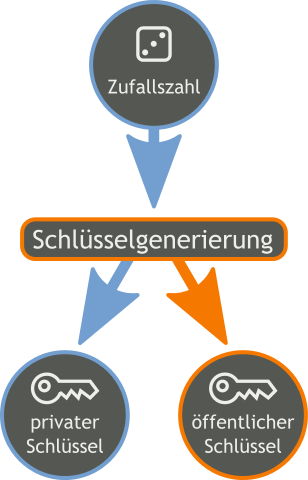
\includegraphics[width=5cm]{abcd.png}	
	\end{center}
	\caption{Erzeugung eines Schlüsselpaars: Blaue Bildelemente sind geheim, orange sind öffentlich.}
	
\end{figure*}

\section{Einwegfunktion}
In der Informatik ist eine Einwegfunktion eine mathematische Funktion, die komplexitätstheoretisch „leicht“ berechenbar, aber „schwer“ umzukehren ist. In einem erweiterten Sinn werden auch Funktionen so bezeichnet, zu denen bisher keine in angemessener Zeit praktisch ausführbare Umkehrung bekannt ist.
Einwegfunktionen bilden die Grundlage asymmetrischer Kryptosysteme.

\section{informationstheoretische Sicherheit}
Perfekte Sicherheit oder auch perfekte Geheimhaltung ist ein von Claude Shannon geprägter Begriff aus der Informationstheorie und Kryptologie. Ein perfekt sicheres Verschlüsselungsverfahren zeichnet sich dadurch aus, dass ein mit ihm erzeugter Schlüsseltext (auch als Geheimtext oder Chiffrat bezeichnet) keinerlei Rückschlüsse auf den korrespondierenden Klartext zulässt. Bei einem solchen Verfahren ist mathematisch bewiesen, dass ein Angreifer, der den Schlüsseltext kennt, abgesehen von der Länge des Klartextes keine weiteren Informationen über diesen gewinnen kann. Er kann den Schlüsseltext also nicht entziffern oder gar das gesamte Verfahren brechen.

\section{RSA-Kryptosystem}
RSA (Rivest, Shamir und Adleman) ist ein asymmetrisches kryptographisches Verfahren, das sowohl zum Verschlüsseln als auch zum digitalen Signieren verwendet werden kann. Es verwendet ein Schlüsselpaar, bestehend aus einem privaten Schlüssel, der zum Entschlüsseln oder Signieren von Daten verwendet wird, und einem öffentlichen Schlüssel, mit dem man verschlüsselt oder Signaturen prüft. Der private Schlüssel wird geheim gehalten und kann nur mit extrem hohem Aufwand aus dem öffentlichen Schlüssel berechnet werden.
%tex root = thesis.tex

\chapter{Praktische Aspeckte}
\label{chapter-aspeckte}
Asymmetrische Kryptosysteme haben den Vorteil, dass sie das Geheimnis möglichst klein halten, da jeder Benutzer nur seinen eigenen privaten Schlüssel geheim halten muss. Im Gegensatz dazu muss bei einem symmetrischen Kryptosystem jeder Benutzer alle Schlüssel geheim halten, was einen mit zunehmender Benutzerzahl steigenden Aufwand bedeutet.\ref{abc}
Im Vergleich zu symmetrischen Algorithmen arbeiten die asymmetrischen Algorithmen sehr langsam. In der Praxis wird dieses Problem auf unterschiedliche Weise umgangen. Zur Verschlüsselung werden hybride Verfahren eingesetzt, bei denen lediglich ein symmetrischer Schlüssel mit dem asymmetrischen Verfahren verschlüsselt wird und die eigentliche Nachricht mit diesem symmetrischen Schlüssel. Bei digitalen Signaturen wird in der Regel statt einer Nachricht nur deren Hashwert signiert.\ref{abcd}
\begin{figure*}
	\label{abc}
	\begin{center}
		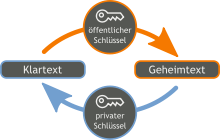
\includegraphics[width=5cm]{abcde.png}	
	\end{center}
	\caption{Verschlüsselung mit öffentlichem Schlüssel und Entschlüsselung mit privatem Schlüssel}
	
\end{figure*}
\begin{figure*}
	\label{abcd}
	\begin{center}
		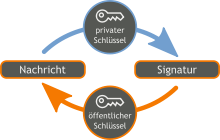
\includegraphics[width=5cm]{ab.png}	
	\end{center}
	\caption{Signieren mit privatem Schlüssel und Verifikation mit öffentlichem Schlüssel}
	
\end{figure*}


\section{Hybride Verschlüsselung}
Unter Hybrider Verschlüsselung versteht man eine Kombination aus asymmetrischer Verschlüsselung und symmetrischer Verschlüsselung. Dabei wählt der Sender einen zufälligen symmetrischen Schlüssel, der Session-Key genannt wird. Mit diesem Session-Key werden die zu schützenden Daten symmetrisch verschlüsselt. Anschließend wird der Session-Key asymmetrisch mit dem öffentlichen Schlüssel des Empfängers verschlüsselt. Dieses Vorgehen löst das Schlüsselverteilungsproblem und erhält dabei den Geschwindigkeitsvorteil der symmetrischen Verschlüsselung.

\section{Hashwert}
Eine kryptologische Hashfunktion oder kryptographische Hashfunktion ist eine spezielle Form der Hashfunktion, welche kollisionsresistent sein sollte und nach Definition immer eine Einwegfunktion ist.
Eine Hashfunktion ist eine Funktion, die eine Zeichenfolge beliebiger Länge auf eine Zeichenfolge mit fester Länge abbildet. Mathematisch ist diese Funktion nicht injektiv (linkseindeutig) und nicht notwendigerweise surjektiv (rechtstotal).
Anwendungen von kryptologischen Hashfunktionen sind vor allem die Datenverarbeitung, zur Integritätsprüfung von Dateien oder Nachrichten. Darüber hinaus werden sie eingesetzt zur Verschleierung von Passwortdateien, als Datenbasis digitaler Signaturen, als Pseudo-Zufallszahlengeneratoren oder zur Konstruktion von Blockchiffren.
Inhaltsverzeichnis.



%! TEX root = thesis.tex

\chapter{Geschichte}
\label{chapter-geschichte}
Den ersten Schritt zur Entwicklung asymmetrischer Verfahren machte Ralph Merkle 1974 mit dem nach ihm benannten Merkles Puzzle, das aber erst 1978 veröffentlicht wurde. Unter dem Einfluss dieser Arbeit entwickelten Whitfield Diffie und Martin Hellman im Jahr 1976 den Diffie-Hellman-Schlüsselaustausch.\cite{ndic} Im Sommer 1975 veröffentlichten Diffie und Hellman eine Idee zur asymmetrischen Verschlüsselung, ohne jedoch ein genaues Verfahren zu kennen. Das erste asymmetrische Verschlüsselungsverfahren wurde 1977 von Ronald L. Rivest, Adi Shamir und Leonard M. Adleman entwickelt und nach ihnen RSA-Verfahren genannt. Nach heutiger Terminologie ist dieses Verfahren eine Falltürpermutation, die sowohl zur Konstruktion von Verschlüsselungsverfahren als auch von Signaturverfahren eingesetzt werden kann.
Unabhängig von den Entwicklungen in der wissenschaftlichen Kryptologie wurde Anfang der 1970er Jahre von drei Mitarbeitern des britischen Government Communications Headquarters, James H. Ellis, Clifford Cocks und Malcolm Williamson, sowohl ein dem späteren Diffie-Hellman-Schlüsselaustausch als auch ein dem RSA-Kryptosystem ähnliches asymmetrisches Verfahren entwickelt, welches aber aus Geheimhaltungsgründen nicht publiziert und auch nicht zum Patent angemeldet wurde.\ref{pa}
\begin{table} 
\caption{Pantentanmeldung}
\label{pa}
 \begin{tabular}{c|l}
  \rowcolor{gray!20}Jahr & Kryptosystem \\\hline
1977&	RSA\\
1978&	Merkle-Hellman\\
1978&	McEliece\\
1979&	Rabin\\
1984	&Chor-Rivest\\
1985&	Elgamal\\

 \end{tabular}
\end{table}
\chapter{Anwendungen}
\label{chapter-anwendungen}
Asymmetrisches Kryptosystem“ ist ein Oberbegriff für Public-Key-Verschlüsselungsverfahren, Public-Key-Authentifizierung und digitale Signaturen. Diese Verfahren werden heutzutage z. B. im E-Mail-Verkehr (OpenPGP, S/MIME) ebenso wie in kryptografischen Protokollen wie SSH oder SSL/TLS verwendet. In größerem Umfang eingesetzt wird beispielsweise das Protokoll https zur sicheren Kommunikation eines Web-Browsers mit einem Server.
Zur Verschlüsselung wird der öffentliche Schlüssel auf den zu verschlüsselnden Text angewandt. Der verschlüsselte Text wird dann vom Schlüsselinhaber mit dem privaten Schlüssel wieder entschlüsselt.
Digitale Signaturen werden u. a. zur sicheren Abwicklung von Geschäften im Internet eingesetzt. Hier ermöglichen sie die Prüfung der Identität der Vertragspartner und der Unverfälschtheit der ausgetauschten Daten (Elektronische Signatur). Dazu ist meist noch eine Public-Key-Infrastruktur notwendig, die die Gültigkeit der verwendeten Schlüssel durch Zertifikate bestätigt.
Zum Erstellen einer Signatur wird ein Hashwert aus der zu verschickenden Nachricht gebildet und mit dem privaten Schlüssel signiert. Nachricht und Signatur werden dann zum Empfänger geschickt, wobei die eigentliche Nachricht nicht verschlüsselt zu sein braucht, da es sich hierbei um eine Signatur (Schaffen von Integrität und Authentizität) und nicht um Verschlüsselung (Schaffen von Vertraulichkeit) handelt.
Zum Verifizieren der Signatur wird die empfangene Signatur des Hashwertes mit dem öffentlichen Schlüssel geprüft. Ist die Verifizierung erfolgreich, so kann davon ausgegangen werden, dass die Nachricht vom Besitzer des privaten Schlüssels stammt und dass die Nachricht bei der Übertragung nicht manipuliert wurde.
\section{Public-Key-Verschlüssungsverfahren}
Ein Public-Key-Verschlüsselungsverfahren ist ein asymmetrisches Verschlüsselungsverfahren, also ein kryptographisches Verfahren, um mit einem öffentlichen Schlüssel einen Klartext in einen Geheimtext umzuwandeln, aus dem der Klartext mit einem geheimen Schlüssel wieder gewonnen werden kann.
Der geheime Schlüssel muss geheim gehalten werden, und es muss praktisch unmöglich sein, ihn aus dem öffentlichen Schlüssel zu berechnen. Der öffentliche Schlüssel muss jedem zugänglich sein, der eine verschlüsselte Nachricht an den Besitzer des geheimen Schlüssels senden will. Dabei muss sichergestellt sein, dass der öffentliche Schlüssel auch wirklich dem Empfänger zugeordnet ist.
\section{Public-Key-Authentifizierung}
Die Public-Key-Authentifizierung ist eine Authentifizierungsmethode, die unter anderem von SSH und OpenSSH verwendet wird, um Benutzer mit Hilfe eines Schlüsselpaars, bestehend aus privatem und öffentlichem Schlüssel, an einem Server anzumelden. Ein solches Schlüsselpaar ist wesentlich schwerer zu kompromittieren als ein Kennwort.
Bei einer Authentifizierung mittels eines Kennworts wird dieses Kennwort, oder dessen Hash-Wert, auf einem Server gespeichert. Hat jemand Zugang zur Kennwortdatei auf diesem Server, gelangt er damit im ersten Fall auch in den Besitz des Kennworts. Im zweiten Fall kann er, mit Hilfe entsprechender Software, eine Zeichenkombination finden, die den gleichen Hash-Wert wie das Kennwort ergibt. Wird das gleiche Kennwort zur Anmeldung auf mehreren Systemen benutzt, so sind damit alle diese Systeme kompromittiert.
Im Gegensatz dazu wird bei der Public-Key-Authentifizierung nur der öffentliche Schlüssel auf einem Server gespeichert. Der private Schlüssel wird auf dem eigenen Rechner gespeichert, kann damit geheim gehalten und zusätzlich mit einer Kennung verschlüsselt werden. Die Kennung kann aus mehreren Wörtern bestehen (im Englischen passphrase).
Die Berechnung des privaten Schlüssels aus dem öffentlichen ist je nach Wahl der Länge des Schlüssels sehr aufwändig bis praktisch unmöglich.
Der öffentliche Schlüssel kann auch zur automatischen Anmeldung (Authentifizierung) genutzt werden. Dabei entfällt der interaktive Dialog zur Kennworteingabe. Hierzu wird auf der User-Seite mit Hilfe seines privaten Schlüssels eine Signatur erzeugt, welche daraufhin auf der Server-Seite mit dem dort hinterlegten öffentlichen Schlüssel des Users verifiziert wird.[1] Das ermöglicht eine Anmeldung in ohne Benutzereingabe ablaufenden Skripten, und beim automatisierten Kopieren von Dateien, beispielsweise mit Secure Copy.
\section{digitale Signatur}
Eine digitale Signatur, auch digitales Signaturverfahren, ist ein asymmetrisches Kryptosystem, bei dem ein Sender mit Hilfe eines geheimen Signaturschlüssels (dem Private Key) zu einer digitalen Nachricht (d. h. zu beliebigen Daten) einen Wert berechnet, der ebenfalls digitale Signatur genannt wird. Dieser Wert ermöglicht es jedem, mit Hilfe des öffentlichen Verifikationsschlüssels (dem Public Key) die nichtabstreitbare Urheberschaft und Integrität der Nachricht zu prüfen. Um eine mit einem Signaturschlüssel erstellte Signatur einer Person zuordnen zu können, muss der zugehörige Verifikationsschlüssel dieser Person zweifelsfrei zugeordnet sein.
\section{SSH}
Secure Shell oder SSH bezeichnet sowohl ein Netzwerkprotokoll als auch entsprechende Programme, mit deren Hilfe man auf eine sichere Art und Weise eine verschlüsselte Netzwerkverbindung mit einem entfernten Gerät herstellen kann. Häufig wird diese Methode verwendet, um lokal eine entfernte Kommandozeile verfügbar zu machen, das heißt, auf einer lokalen Konsole werden die Ausgaben der entfernten Konsole ausgegeben und die lokalen Tastatureingaben werden an den entfernten Rechner gesendet. Genutzt werden kann dies beispielsweise zur Fernwartung eines in einem entfernten Rechenzentrum stehenden Servers. Die neuere Protokoll-Version SSH-2 bietet weitere Funktionen wie Datenübertragung per SFTP.
%! TEX root = thesis.tex
\chapter{Zusammenfassung}
Ein asymmetrisches Kryptosystem oder Public-Key-Kryptosystem ist ein kryptographisches Verfahren, bei dem im Gegensatz zu einem symmetrischen Kryptosystem die kommunizierenden Parteien keinen gemeinsamen geheimen Schlüssel zu kennen brauchen. Jeder Benutzer erzeugt sein eigenes Schlüsselpaar, das aus einem geheimen Teil (privater Schlüssel) und einem nicht geheimen Teil (öffentlicher Schlüssel) besteht. Der öffentliche Schlüssel ermöglicht es jedem, Daten für den Besitzer des privaten Schlüssels zu verschlüsseln, dessen digitale Signaturen zu prüfen oder ihn zu authentifizieren. Der private Schlüssel ermöglicht es seinem Besitzer, mit dem öffentlichen Schlüssel verschlüsselte Daten zu entschlüsseln, digitale Signaturen zu erzeugen oder sich zu authentisieren.
Im folgenden weitere Literatur in Form von Büchern genannt\cite{krsog}, \cite{gb}, \cite{ak}.
Der noch fehlende Bericht in einen Konferenzband \cite{DBLP:conf/pkc/BernhardFW16}.

 \cleardoublepage
\phantomsection
\pdfbookmark{Abbildungsverzeichnis}{listoffigures}
\listoffigures

\cleardoublepage
\phantomsection
\pdfbookmark{Tabellenverzeichnis}{listoftables}
\listoftables

\cleardoublepage
\phantomsection
\pdfbookmark{Definitions- und Theoremverzeichnis}{listoftheorems}
\renewcommand{\listtheoremname}{Definitions- und Theoremverzeichnis}
\listoftheorems[ignoreall,show={Lemma,Theorem,Korollar,Definition}]

\backmatter
\cleardoublepage
\phantomsection
\pdfbookmark{Literaturverzeichnis}{bibliography}
\bibliography{literature}
\end{document}